% Options for packages loaded elsewhere
\PassOptionsToPackage{unicode}{hyperref}
\PassOptionsToPackage{hyphens}{url}
\PassOptionsToPackage{dvipsnames,svgnames,x11names}{xcolor}
%
\documentclass[
]{article}
\usepackage{amsmath,amssymb}
\usepackage{iftex}
\ifPDFTeX
  \usepackage[T1]{fontenc}
  \usepackage[utf8]{inputenc}
  \usepackage{textcomp} % provide euro and other symbols
\else % if luatex or xetex
  \usepackage{unicode-math} % this also loads fontspec
  \defaultfontfeatures{Scale=MatchLowercase}
  \defaultfontfeatures[\rmfamily]{Ligatures=TeX,Scale=1}
\fi
\usepackage{lmodern}
\ifPDFTeX\else
  % xetex/luatex font selection
\fi
% Use upquote if available, for straight quotes in verbatim environments
\IfFileExists{upquote.sty}{\usepackage{upquote}}{}
\IfFileExists{microtype.sty}{% use microtype if available
  \usepackage[]{microtype}
  \UseMicrotypeSet[protrusion]{basicmath} % disable protrusion for tt fonts
}{}
\makeatletter
\@ifundefined{KOMAClassName}{% if non-KOMA class
  \IfFileExists{parskip.sty}{%
    \usepackage{parskip}
  }{% else
    \setlength{\parindent}{0pt}
    \setlength{\parskip}{6pt plus 2pt minus 1pt}}
}{% if KOMA class
  \KOMAoptions{parskip=half}}
\makeatother
\usepackage{xcolor}
\usepackage[margin=1in]{geometry}
\usepackage{color}
\usepackage{fancyvrb}
\newcommand{\VerbBar}{|}
\newcommand{\VERB}{\Verb[commandchars=\\\{\}]}
\DefineVerbatimEnvironment{Highlighting}{Verbatim}{commandchars=\\\{\}}
% Add ',fontsize=\small' for more characters per line
\usepackage{framed}
\definecolor{shadecolor}{RGB}{248,248,248}
\newenvironment{Shaded}{\begin{snugshade}}{\end{snugshade}}
\newcommand{\AlertTok}[1]{\textcolor[rgb]{0.94,0.16,0.16}{#1}}
\newcommand{\AnnotationTok}[1]{\textcolor[rgb]{0.56,0.35,0.01}{\textbf{\textit{#1}}}}
\newcommand{\AttributeTok}[1]{\textcolor[rgb]{0.13,0.29,0.53}{#1}}
\newcommand{\BaseNTok}[1]{\textcolor[rgb]{0.00,0.00,0.81}{#1}}
\newcommand{\BuiltInTok}[1]{#1}
\newcommand{\CharTok}[1]{\textcolor[rgb]{0.31,0.60,0.02}{#1}}
\newcommand{\CommentTok}[1]{\textcolor[rgb]{0.56,0.35,0.01}{\textit{#1}}}
\newcommand{\CommentVarTok}[1]{\textcolor[rgb]{0.56,0.35,0.01}{\textbf{\textit{#1}}}}
\newcommand{\ConstantTok}[1]{\textcolor[rgb]{0.56,0.35,0.01}{#1}}
\newcommand{\ControlFlowTok}[1]{\textcolor[rgb]{0.13,0.29,0.53}{\textbf{#1}}}
\newcommand{\DataTypeTok}[1]{\textcolor[rgb]{0.13,0.29,0.53}{#1}}
\newcommand{\DecValTok}[1]{\textcolor[rgb]{0.00,0.00,0.81}{#1}}
\newcommand{\DocumentationTok}[1]{\textcolor[rgb]{0.56,0.35,0.01}{\textbf{\textit{#1}}}}
\newcommand{\ErrorTok}[1]{\textcolor[rgb]{0.64,0.00,0.00}{\textbf{#1}}}
\newcommand{\ExtensionTok}[1]{#1}
\newcommand{\FloatTok}[1]{\textcolor[rgb]{0.00,0.00,0.81}{#1}}
\newcommand{\FunctionTok}[1]{\textcolor[rgb]{0.13,0.29,0.53}{\textbf{#1}}}
\newcommand{\ImportTok}[1]{#1}
\newcommand{\InformationTok}[1]{\textcolor[rgb]{0.56,0.35,0.01}{\textbf{\textit{#1}}}}
\newcommand{\KeywordTok}[1]{\textcolor[rgb]{0.13,0.29,0.53}{\textbf{#1}}}
\newcommand{\NormalTok}[1]{#1}
\newcommand{\OperatorTok}[1]{\textcolor[rgb]{0.81,0.36,0.00}{\textbf{#1}}}
\newcommand{\OtherTok}[1]{\textcolor[rgb]{0.56,0.35,0.01}{#1}}
\newcommand{\PreprocessorTok}[1]{\textcolor[rgb]{0.56,0.35,0.01}{\textit{#1}}}
\newcommand{\RegionMarkerTok}[1]{#1}
\newcommand{\SpecialCharTok}[1]{\textcolor[rgb]{0.81,0.36,0.00}{\textbf{#1}}}
\newcommand{\SpecialStringTok}[1]{\textcolor[rgb]{0.31,0.60,0.02}{#1}}
\newcommand{\StringTok}[1]{\textcolor[rgb]{0.31,0.60,0.02}{#1}}
\newcommand{\VariableTok}[1]{\textcolor[rgb]{0.00,0.00,0.00}{#1}}
\newcommand{\VerbatimStringTok}[1]{\textcolor[rgb]{0.31,0.60,0.02}{#1}}
\newcommand{\WarningTok}[1]{\textcolor[rgb]{0.56,0.35,0.01}{\textbf{\textit{#1}}}}
\usepackage{graphicx}
\makeatletter
\def\maxwidth{\ifdim\Gin@nat@width>\linewidth\linewidth\else\Gin@nat@width\fi}
\def\maxheight{\ifdim\Gin@nat@height>\textheight\textheight\else\Gin@nat@height\fi}
\makeatother
% Scale images if necessary, so that they will not overflow the page
% margins by default, and it is still possible to overwrite the defaults
% using explicit options in \includegraphics[width, height, ...]{}
\setkeys{Gin}{width=\maxwidth,height=\maxheight,keepaspectratio}
% Set default figure placement to htbp
\makeatletter
\def\fps@figure{htbp}
\makeatother
\setlength{\emergencystretch}{3em} % prevent overfull lines
\providecommand{\tightlist}{%
  \setlength{\itemsep}{0pt}\setlength{\parskip}{0pt}}
\setcounter{secnumdepth}{5}
\usepackage[french]{babel}
\ifLuaTeX
  \usepackage{selnolig}  % disable illegal ligatures
\fi
\usepackage{bookmark}
\IfFileExists{xurl.sty}{\usepackage{xurl}}{} % add URL line breaks if available
\urlstyle{same}
\hypersetup{
  pdfauthor={Vincent Runge},
  colorlinks=true,
  linkcolor={Maroon},
  filecolor={Maroon},
  citecolor={Blue},
  urlcolor={blue},
  pdfcreator={LaTeX via pandoc}}

\title{Evaluation des algorithmes heuristiques pour le voyageur de
commerce\\

\includegraphics[width=1in,height=\textheight]{Images/logo_lamme.png}

\includegraphics[width=1.7in,height=\textheight]{Images/logo_UEVE.png}\\
\strut ~M2 Data Science Algorithmique}
\author{Vincent Runge}
\date{vendredi 14 mars 2025}

\begin{document}
\maketitle

{
\hypersetup{linkcolor=}
\setcounter{tocdepth}{2}
\tableofcontents
}
\noindent\hrulefill

\section{Description du problème et
objectif}\label{description-du-probluxe8me-et-objectif}

On tire de manière aléatoire dans le carré unité selon une loi uniforme
\(\mathcal{U}(0,1) \times \mathcal{U}(0,1)\) un nombre \texttt{n} de
villes. On donne ici un exemple avec 40 villes :

\begin{Shaded}
\begin{Highlighting}[]
\NormalTok{n }\OtherTok{\textless{}{-}} \DecValTok{40}
\NormalTok{villes }\OtherTok{\textless{}{-}} \FunctionTok{matrix}\NormalTok{(}\FunctionTok{runif}\NormalTok{(}\DecValTok{2}\SpecialCharTok{*}\NormalTok{n), n, }\DecValTok{2}\NormalTok{)}
\end{Highlighting}
\end{Shaded}

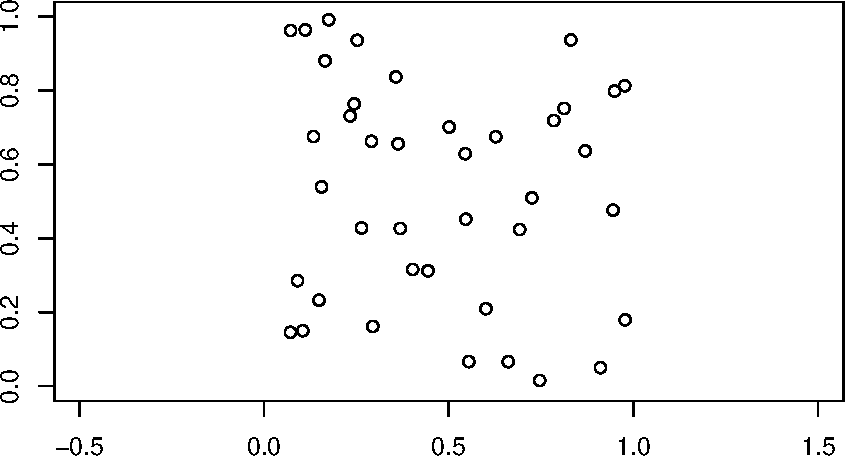
\includegraphics{TSP_analyse_files/figure-latex/unnamed-chunk-2-1.pdf}

Notre premier objectif est de contruire un ``plus court chemin'' par un
\textbf{algorithme heuristique}. On comparera différentes
\textbf{méthodes d'insertion} et on analysera leur \textbf{temps de
calcul} numériquement.

\textbf{Notre objectif (TP) : }

\begin{itemize}
\item
  comparer les performances en temps des algorithmes
\item
  évaluer la distance à la solution optimale
\item
  pour cela coder les algorithmes exacts de \emph{branch and bound} et
  \emph{Held Karp}.
\end{itemize}

On note \(c(i,j)\) le coût pour passer de la ville \(i\) à la ville
\(j\). Notre objectif est de trouver la permutation des indices
\((1,...,n)\) notée \((v_1,...,v_n)\) qui minimisera la longueur du
tour:

\[\sum_{i=1}^{n}c(v_i,v_{i+1})\] avec \(v_{n+1} = v_1\). Remarquez bien
qu'une permutation contient une et une seule fois chaque indice de sorte
que le tour est complet et passe bien par chaque ville une et une seule
fois. Le coût \(c(i,j)\) sera dans ce document égal à la distance
euclidienne.

\section{L'algorithme naïf du plus proche
voisin}\label{lalgorithme-nauxeff-du-plus-proche-voisin}

C'est la méthode la plus simple. Elle consiste à partir d'une ville
\(i\) et de contruire le chemin de proche en proche en ajoutant en bout
de chemin la ville la plus proche parmi les villes non explorées. Quand
toutes les villes sont explorées on revient à la première ville pour
fermer le tour.

On peut répéter la procédure pour chaque ville de départ (on exécute
ainsi \(n\) fois cette méthode) pour choisir le meilleur chemin parmi
les \(n\) obtenus.

(librairies à installer)

\begin{Shaded}
\begin{Highlighting}[]
\FunctionTok{library}\NormalTok{(ggplot2) }\CommentTok{\#ggplot}
\FunctionTok{library}\NormalTok{(reshape2) }\CommentTok{\#melt}
\FunctionTok{library}\NormalTok{(parallel) }\CommentTok{\#mclapply}
\end{Highlighting}
\end{Shaded}

\begin{Shaded}
\begin{Highlighting}[]
\FunctionTok{library}\NormalTok{(M2algorithmique)}
\NormalTok{res1 }\OtherTok{\textless{}{-}} \FunctionTok{TSP\_naif}\NormalTok{(villes, }\AttributeTok{type =} \StringTok{"one"}\NormalTok{)}
\end{Highlighting}
\end{Shaded}

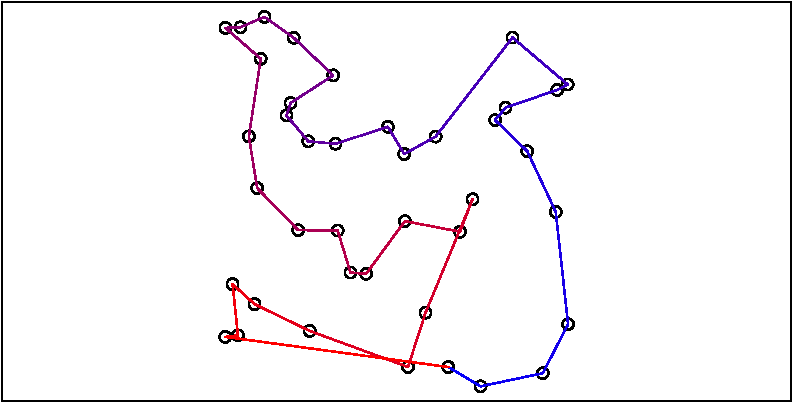
\includegraphics{TSP_analyse_files/figure-latex/unnamed-chunk-5-1.pdf}

\begin{verbatim}
## [1] 5.808868
\end{verbatim}

\begin{verbatim}
## Longueur = 5.808868
\end{verbatim}

\begin{center}\rule{0.5\linewidth}{0.5pt}\end{center}

\textbf{Exercice :} pour le problème euclidien du voyageur de commerce
(inégalité triangulaire respectée), le tour optimal ne peut pas contenir
de croisement.

En effet, supposons que le tour contienne un croisement. Cela signifie
qu'il existe quatre villes A,B,C,D telles que les arêtes (A,C) et (B,D)
se croisent. On échange les arêtes croisées: connecter A à B puis C à D.
Cela supprime le croisement.

Si AC et BD se coupent en O. On a :

\[d(A,B) \le d(A,O) + d(O,B) \,,\quad d(C,D) \le d(C,O) + d(O,D) \] donc

\[d(A,B) + d(C,D) \le d(A,O) + d(O,B) + d(C,O) + d(O,D) = d(A,C) + d(B,D)\]
Dans le tour, \(A => C\) et \(B => D\) est remplacé par \(A => B\) et
\(C => D\), l'entrée par \(A\) et la sortie par \(D\) sont respectés.
Tout autre permutation des lettres est possible et mène au même résultat

\begin{center}\rule{0.5\linewidth}{0.5pt}\end{center}

\section{Les algorithmes d'insertion}\label{les-algorithmes-dinsertion}

les algorithmes d'insertion consistent à insérer les villes les unes
après les autres \textbf{dans un tour partiel} (contenant qu'un
sous-ensemble des villes) partant d'une ou deux villes de départ.

\subsection{\texorpdfstring{L'algorithme d'insertion \emph{cheapest}
(``le moins
cher'')}{L'algorithme d'insertion cheapest (``le moins cher'')}}\label{lalgorithme-dinsertion-cheapest-le-moins-cher}

Pour un tour partiel déjà constitué on cherche l'arrête (le couple de
villes) \((i,j)\) et la ville encore non incluse \(k\) qui minimise la
quantité

\[c(i,k) + c(k,j) - c(i,j)\] C'est ainsi l'insertion la moins coûteuse.
On pourra aussi répéter l'algorithme pour chacune des villes de départ.

\begin{Shaded}
\begin{Highlighting}[]
\NormalTok{res2 }\OtherTok{\textless{}{-}} \FunctionTok{TSP\_cheapest}\NormalTok{(villes, }\AttributeTok{type =} \StringTok{"one"}\NormalTok{)}
\end{Highlighting}
\end{Shaded}

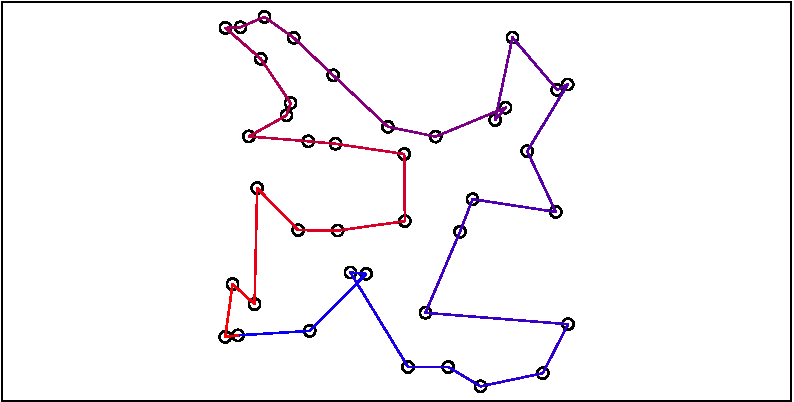
\includegraphics{TSP_analyse_files/figure-latex/unnamed-chunk-7-1.pdf}

\begin{verbatim}
## [1] 5.921506
\end{verbatim}

\begin{verbatim}
## Longueur = 5.921506
\end{verbatim}

\subsection{\texorpdfstring{L'algorithme d'insertion \emph{nearest}
(``le plus
proche'')}{L'algorithme d'insertion nearest (``le plus proche'')}}\label{lalgorithme-dinsertion-nearest-le-plus-proche}

Pour un tour partiel déjà constitué on cherche la ville \(i\) et la
ville encore non incluse \(k\) qui minimise la quantité \(c(i,k)\) :
c'est la ville la plus proche du tour. Une fois trouvée on insert cette
ville à sa position optimale en trouvant l'arrête \((i,j)\) qui minimise
\(c(i,k) + c(k,j) - c(i,j)\) C'est ainsi l'insertion la plus proche. On
pourra aussi répéter l'algorithme pour chacune des villes de départ.

\begin{Shaded}
\begin{Highlighting}[]
\NormalTok{res3 }\OtherTok{\textless{}{-}} \FunctionTok{TSP\_nearest}\NormalTok{(villes)}
\end{Highlighting}
\end{Shaded}

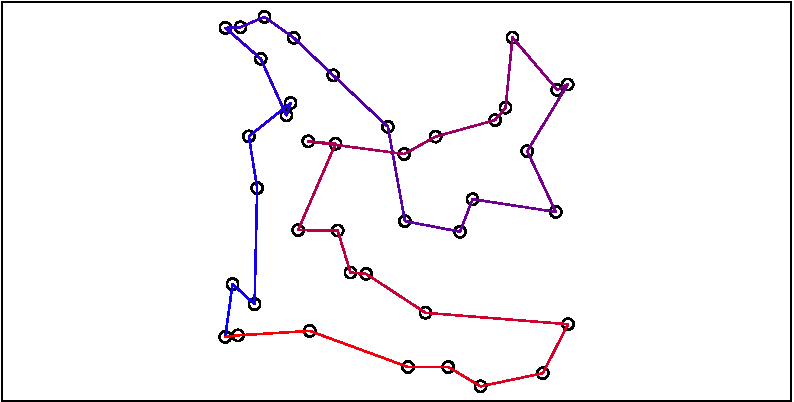
\includegraphics{TSP_analyse_files/figure-latex/unnamed-chunk-9-1.pdf}

\begin{verbatim}
## [1] 5.89975
\end{verbatim}

\begin{verbatim}
## Longueur = 5.89975
\end{verbatim}

\subsection{\texorpdfstring{L'algorithme d'insertion \emph{farthest}
(``le plus
éloigné'')}{L'algorithme d'insertion farthest (``le plus éloigné'')}}\label{lalgorithme-dinsertion-farthest-le-plus-uxe9loignuxe9}

Pour un tour partiel déjà constitué on cherche pour chaque ville non
encore incluse \(k\), la ville \(i\) du tour la plus proche. On obtient
des distances \(c(i,k)\) avec autant de couples \((i,k)\) qu'il y a de
villes non incluses. On sélectionne le plus grande de ces distances et
la ville \(k\) qui lui est associée. On insère cette ville \(k\) à sa
position optimale selon le critère habituel (min de
\(c(i,k) + c(k,j) - c(i,j)\)).

\begin{Shaded}
\begin{Highlighting}[]
\NormalTok{res4 }\OtherTok{\textless{}{-}} \FunctionTok{TSP\_farthest}\NormalTok{(villes)}
\end{Highlighting}
\end{Shaded}

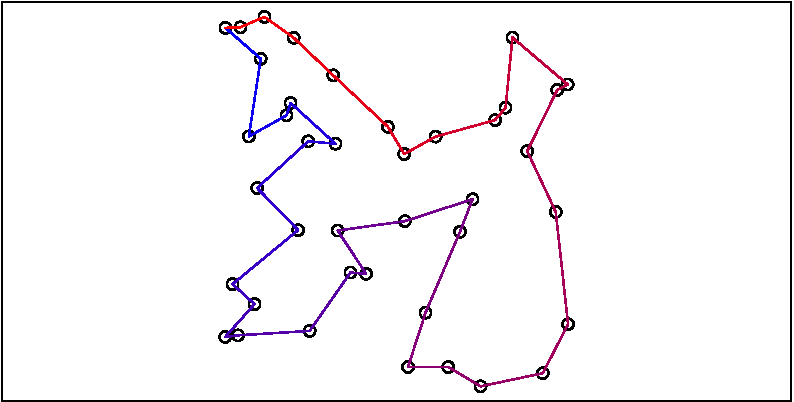
\includegraphics{TSP_analyse_files/figure-latex/unnamed-chunk-11-1.pdf}

\begin{verbatim}
## [1] 5.418704
\end{verbatim}

\begin{verbatim}
## Longueur = 5.418704
\end{verbatim}

Affichés tous ensemble :

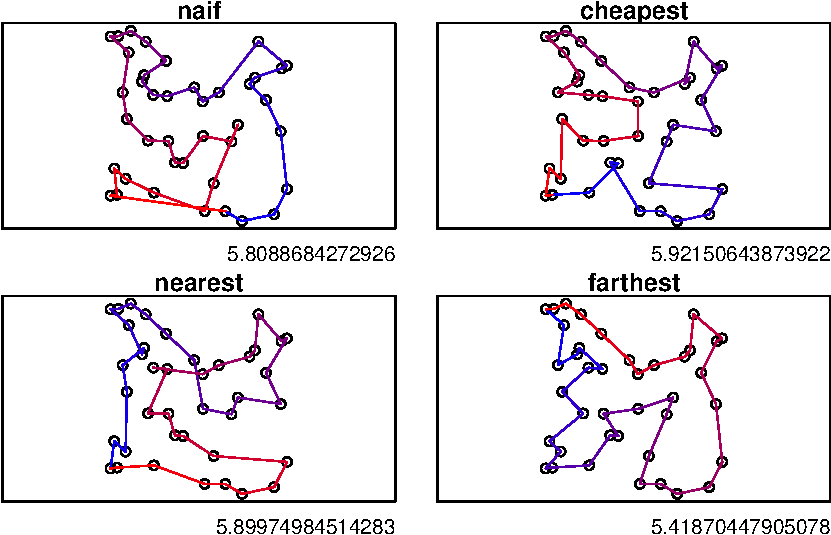
\includegraphics{TSP_analyse_files/figure-latex/unnamed-chunk-12-1.pdf}

Il est possible dans ce cadre eucliden d'obtenir une
\href{https://www.researchgate.net/publication/220616869_An_Analysis_of_Several_Heuristics_for_the_Traveling_Salesman_Problem}{bornes
sur la longueur du tour}. Ces algorithmes heuristiques sont donc des
algorithmes d'approximation (sauf peut-être pour \emph{farthest})!

\[algo(cheapest) \le 2 \,algo(opt)\]

\[algo(nearest) \le 2 \,algo(opt)\]

\[algo(farthest) \le (\lceil log_2(n) \rceil + 1) \,algo(opt)\]

\section{Comparaison des
performances}\label{comparaison-des-performances}

\subsection{Pour les différents algorithmes
heuristiques}\label{pour-les-diffuxe9rents-algorithmes-heuristiques}

On répète 100 fois les 4 algorithmes sur des données générées par
\(\mathcal{U}[0,1] \times \mathcal{U}[0,1]\)

\begin{verbatim}
## No id variables; using all as measure variables
\end{verbatim}

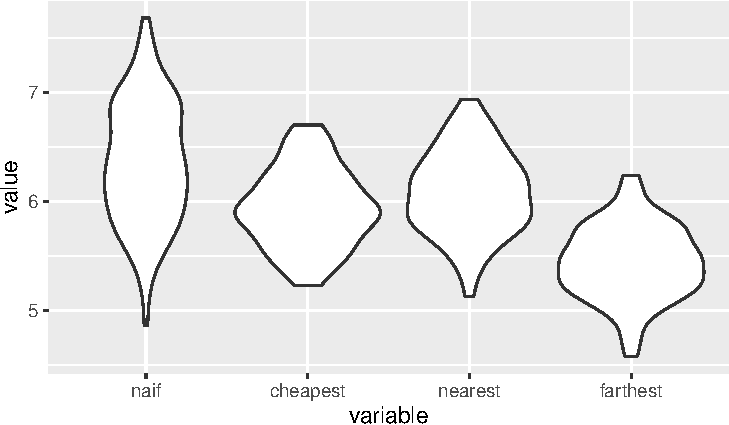
\includegraphics{TSP_analyse_files/figure-latex/unnamed-chunk-13-1.pdf}

Rang moyen :

\begin{verbatim}
##     naif cheapest  nearest farthest 
##     3.46     2.51     2.99     1.04
\end{verbatim}

\subsection{Pour une distribution normale des
villes}\label{pour-une-distribution-normale-des-villes}

On répète 100 fois les 4 algorithmes sur des données normales générées
par \(\mathcal{N}(0,1) \times \mathcal{N}(0,1)\)

\begin{verbatim}
## No id variables; using all as measure variables
\end{verbatim}

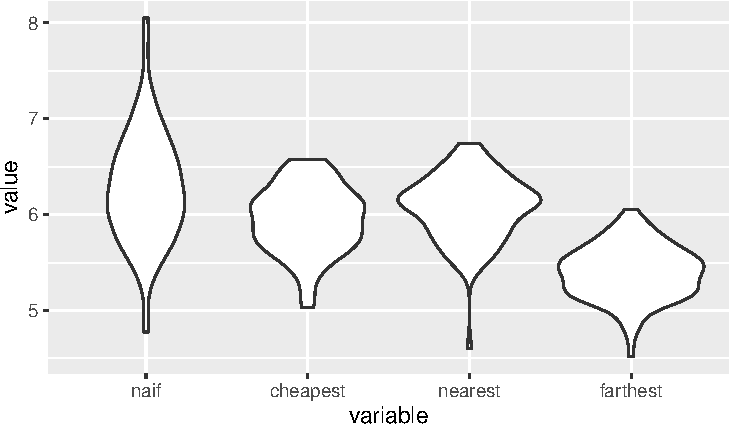
\includegraphics{TSP_analyse_files/figure-latex/unnamed-chunk-15-1.pdf}

Rang moyen :

\begin{verbatim}
##     naif cheapest  nearest farthest 
##     3.31     2.59     3.04     1.06
\end{verbatim}

Comment évoluent ces résultats si on répète chaque algorithme pour les
\(n\) initialisations possibles? Avec la distribution uniforme des
villes on obtient:

\begin{verbatim}
## No id variables; using all as measure variables
\end{verbatim}

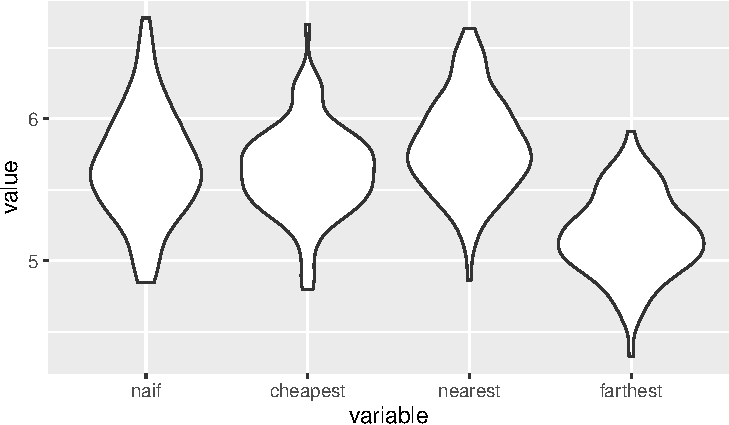
\includegraphics{TSP_analyse_files/figure-latex/unnamed-chunk-17-1.pdf}

Rang moyen :

\begin{verbatim}
##     naif cheapest  nearest farthest 
##     2.85     2.68     3.47     1.00
\end{verbatim}

\section{Temps de calcul}\label{temps-de-calcul}

On étudie ici le temps la complexité des algorithmes en fonction du
nombre \(n\) de villes.

On définit une fonction de type \texttt{one.simu} qui simule une seule
expérience pour un choix de ville.

\begin{Shaded}
\begin{Highlighting}[]
\NormalTok{one.simu\_time\_TSP }\OtherTok{\textless{}{-}} \ControlFlowTok{function}\NormalTok{(i, data, }\AttributeTok{algo =} \StringTok{"naif"}\NormalTok{, }\AttributeTok{type =} \StringTok{"one"}\NormalTok{)}
\NormalTok{\{}
  \ControlFlowTok{if}\NormalTok{(algo }\SpecialCharTok{==} \StringTok{"naif"}\NormalTok{)}
\NormalTok{  \{}
\NormalTok{    start\_time }\OtherTok{\textless{}{-}} \FunctionTok{Sys.time}\NormalTok{()}
    \FunctionTok{TSP\_naif}\NormalTok{(data, }\AttributeTok{type =}\NormalTok{ type)}
\NormalTok{    end\_time  }\OtherTok{\textless{}{-}} \FunctionTok{Sys.time}\NormalTok{()}
\NormalTok{  \}}
  \ControlFlowTok{if}\NormalTok{(algo }\SpecialCharTok{==} \StringTok{"cheapest"}\NormalTok{)}
\NormalTok{  \{}
\NormalTok{    start\_time }\OtherTok{\textless{}{-}} \FunctionTok{Sys.time}\NormalTok{()}
    \FunctionTok{TSP\_cheapest}\NormalTok{(data, }\AttributeTok{type =}\NormalTok{ type)}
\NormalTok{    end\_time  }\OtherTok{\textless{}{-}} \FunctionTok{Sys.time}\NormalTok{()}
\NormalTok{  \}}
  \ControlFlowTok{if}\NormalTok{(algo }\SpecialCharTok{==} \StringTok{"nearest"}\NormalTok{)}
\NormalTok{  \{}
\NormalTok{    start\_time }\OtherTok{\textless{}{-}} \FunctionTok{Sys.time}\NormalTok{()}
    \FunctionTok{TSP\_nearest}\NormalTok{(data, }\AttributeTok{type =}\NormalTok{ type)}
\NormalTok{    end\_time  }\OtherTok{\textless{}{-}} \FunctionTok{Sys.time}\NormalTok{()}
\NormalTok{  \}}
  \ControlFlowTok{if}\NormalTok{(algo }\SpecialCharTok{==} \StringTok{"farthest"}\NormalTok{)}
\NormalTok{  \{}
\NormalTok{    start\_time }\OtherTok{\textless{}{-}} \FunctionTok{Sys.time}\NormalTok{()}
    \FunctionTok{TSP\_farthest}\NormalTok{(data, }\AttributeTok{type =}\NormalTok{ type)}
\NormalTok{    end\_time  }\OtherTok{\textless{}{-}} \FunctionTok{Sys.time}\NormalTok{()}
\NormalTok{  \}}
  \FunctionTok{return}\NormalTok{(}\FunctionTok{unclass}\NormalTok{(end\_time }\SpecialCharTok{{-}}\NormalTok{ start\_time)[}\DecValTok{1}\NormalTok{])}
\NormalTok{\}}
\end{Highlighting}
\end{Shaded}

On construit un vecteur contenant \textbf{des tailles croissante de
nombre de villes} selon une échelle logarithmique.

\begin{Shaded}
\begin{Highlighting}[]
\NormalTok{my\_n\_vector\_LOG }\OtherTok{\textless{}{-}} \FunctionTok{seq}\NormalTok{(}\AttributeTok{from =} \FunctionTok{log}\NormalTok{(}\DecValTok{10}\NormalTok{), }\AttributeTok{to =} \FunctionTok{log}\NormalTok{(}\DecValTok{100}\NormalTok{), }\AttributeTok{by =} \FunctionTok{log}\NormalTok{(}\DecValTok{10}\NormalTok{)}\SpecialCharTok{/}\DecValTok{40}\NormalTok{)}
\NormalTok{my\_n\_vector }\OtherTok{\textless{}{-}} \FunctionTok{round}\NormalTok{(}\FunctionTok{exp}\NormalTok{(my\_n\_vector\_LOG))}
\NormalTok{my\_n\_vector}
\end{Highlighting}
\end{Shaded}

\begin{verbatim}
##  [1]  10  11  11  12  13  13  14  15  16  17  18  19  20  21  22  24  25  27  28
## [20]  30  32  33  35  38  40  42  45  47  50  53  56  60  63  67  71  75  79  84
## [39]  89  94 100
\end{verbatim}

\begin{Shaded}
\begin{Highlighting}[]
\FunctionTok{diff}\NormalTok{(}\FunctionTok{log}\NormalTok{(my\_n\_vector))}
\end{Highlighting}
\end{Shaded}

\begin{verbatim}
##  [1] 0.09531018 0.00000000 0.08701138 0.08004271 0.00000000 0.07410797
##  [7] 0.06899287 0.06453852 0.06062462 0.05715841 0.05406722 0.05129329
## [13] 0.04879016 0.04652002 0.08701138 0.04082199 0.07696104 0.03636764
## [19] 0.06899287 0.06453852 0.03077166 0.05884050 0.08223810 0.05129329
## [25] 0.04879016 0.06899287 0.04348511 0.06187540 0.05826891 0.05505978
## [31] 0.06899287 0.04879016 0.06155789 0.05798726 0.05480824 0.05195974
## [37] 0.06136895 0.05781957 0.05465841 0.06187540
\end{verbatim}

On voit que \texttt{diff(log())} est à peu près constant. Ce n'est pas
constant à cause de l'arrondi avec \texttt{round}. On construit un data
frame qui contiendra les résultats :

\begin{Shaded}
\begin{Highlighting}[]
\NormalTok{p }\OtherTok{\textless{}{-}} \DecValTok{50} \DocumentationTok{\#\#\# répétition}
\NormalTok{df }\OtherTok{\textless{}{-}} \FunctionTok{data.frame}\NormalTok{(}\FunctionTok{matrix}\NormalTok{( }\AttributeTok{nrow =} \DecValTok{4} \SpecialCharTok{*} \FunctionTok{length}\NormalTok{(my\_n\_vector), }\AttributeTok{ncol =} \DecValTok{2} \SpecialCharTok{+}\NormalTok{ p))}
\FunctionTok{colnames}\NormalTok{(df) }\OtherTok{\textless{}{-}} \FunctionTok{c}\NormalTok{(}\StringTok{"type"}\NormalTok{, }\StringTok{"n"}\NormalTok{, }\DecValTok{1}\SpecialCharTok{:}\NormalTok{p)}
\FunctionTok{dim}\NormalTok{(df)}
\end{Highlighting}
\end{Shaded}

\begin{verbatim}
## [1] 164  52
\end{verbatim}

On lance la simulation sur plusieurs coeurs.

\begin{Shaded}
\begin{Highlighting}[]
\NormalTok{nbCores }\OtherTok{\textless{}{-}} \DecValTok{8}
\NormalTok{j }\OtherTok{\textless{}{-}} \DecValTok{1}

\ControlFlowTok{for}\NormalTok{(n }\ControlFlowTok{in}\NormalTok{ my\_n\_vector)}
\NormalTok{\{}
  \CommentTok{\#print(n)}
\NormalTok{  liste1 }\OtherTok{\textless{}{-}} \FunctionTok{mclapply}\NormalTok{(}\DecValTok{1}\SpecialCharTok{:}\NormalTok{p, }\AttributeTok{FUN =}\NormalTok{ one.simu\_time\_TSP,}
                      \AttributeTok{data =} \FunctionTok{matrix}\NormalTok{(}\FunctionTok{runif}\NormalTok{(}\DecValTok{2}\SpecialCharTok{*}\NormalTok{n), n, }\DecValTok{2}\NormalTok{),}
                     \AttributeTok{algo =} \StringTok{"naif"}\NormalTok{,}
                     \AttributeTok{mc.cores =}\NormalTok{ nbCores)}

\NormalTok{  liste2 }\OtherTok{\textless{}{-}} \FunctionTok{mclapply}\NormalTok{(}\DecValTok{1}\SpecialCharTok{:}\NormalTok{p, }\AttributeTok{FUN =}\NormalTok{ one.simu\_time\_TSP,}
                     \AttributeTok{data =} \FunctionTok{matrix}\NormalTok{(}\FunctionTok{runif}\NormalTok{(}\DecValTok{2}\SpecialCharTok{*}\NormalTok{n), n, }\DecValTok{2}\NormalTok{),}
                     \AttributeTok{algo =} \StringTok{"cheapest"}\NormalTok{,}
                     \AttributeTok{mc.cores =}\NormalTok{ nbCores)}

\NormalTok{  liste3 }\OtherTok{\textless{}{-}} \FunctionTok{mclapply}\NormalTok{(}\DecValTok{1}\SpecialCharTok{:}\NormalTok{p, }\AttributeTok{FUN =}\NormalTok{ one.simu\_time\_TSP,}
                     \AttributeTok{data =} \FunctionTok{matrix}\NormalTok{(}\FunctionTok{runif}\NormalTok{(}\DecValTok{2}\SpecialCharTok{*}\NormalTok{n), n, }\DecValTok{2}\NormalTok{),}
                     \AttributeTok{algo =} \StringTok{"nearest"}\NormalTok{,}
                     \AttributeTok{mc.cores =}\NormalTok{ nbCores)}

\NormalTok{  liste4 }\OtherTok{\textless{}{-}} \FunctionTok{mclapply}\NormalTok{(}\DecValTok{1}\SpecialCharTok{:}\NormalTok{p, }\AttributeTok{FUN =}\NormalTok{ one.simu\_time\_TSP,}
                     \AttributeTok{data =} \FunctionTok{matrix}\NormalTok{(}\FunctionTok{runif}\NormalTok{(}\DecValTok{2}\SpecialCharTok{*}\NormalTok{n), n, }\DecValTok{2}\NormalTok{),}
                     \AttributeTok{algo =} \StringTok{"farthest"}\NormalTok{,}
                     \AttributeTok{mc.cores =}\NormalTok{ nbCores)}

\NormalTok{  df[j ,] }\OtherTok{\textless{}{-}} \FunctionTok{c}\NormalTok{(}\StringTok{"naif"}\NormalTok{, n, }\FunctionTok{do.call}\NormalTok{(cbind, liste1))}
\NormalTok{  df[j}\SpecialCharTok{+}\DecValTok{1}\NormalTok{ ,] }\OtherTok{\textless{}{-}} \FunctionTok{c}\NormalTok{(}\StringTok{"cheapest"}\NormalTok{, n, }\FunctionTok{do.call}\NormalTok{(cbind, liste2))}
\NormalTok{  df[j}\SpecialCharTok{+}\DecValTok{2}\NormalTok{ ,] }\OtherTok{\textless{}{-}} \FunctionTok{c}\NormalTok{(}\StringTok{"nearest"}\NormalTok{, n, }\FunctionTok{do.call}\NormalTok{(cbind, liste3))}
\NormalTok{  df[j}\SpecialCharTok{+}\DecValTok{3}\NormalTok{ ,] }\OtherTok{\textless{}{-}} \FunctionTok{c}\NormalTok{(}\StringTok{"farthest"}\NormalTok{, n, }\FunctionTok{do.call}\NormalTok{(cbind, liste4))}
\NormalTok{  j }\OtherTok{\textless{}{-}}\NormalTok{ j }\SpecialCharTok{+} \DecValTok{4}
\NormalTok{\}}

\NormalTok{df }\OtherTok{\textless{}{-}} \FunctionTok{melt}\NormalTok{(df, }\AttributeTok{id.vars =} \FunctionTok{c}\NormalTok{(}\StringTok{"type"}\NormalTok{,}\StringTok{"n"}\NormalTok{))}
\end{Highlighting}
\end{Shaded}

tranformations techniques :

\begin{Shaded}
\begin{Highlighting}[]
\NormalTok{data\_summary }\OtherTok{\textless{}{-}} \ControlFlowTok{function}\NormalTok{(data, varname, groupnames)}
\NormalTok{\{}
  \FunctionTok{require}\NormalTok{(plyr)}
\NormalTok{  summary\_func }\OtherTok{\textless{}{-}} \ControlFlowTok{function}\NormalTok{(x, col)}
\NormalTok{  \{}
    \FunctionTok{c}\NormalTok{(}\AttributeTok{mean =} \FunctionTok{mean}\NormalTok{(x[[col]], }\AttributeTok{na.rm=}\ConstantTok{TRUE}\NormalTok{),}
      \AttributeTok{q1 =} \FunctionTok{quantile}\NormalTok{(x[[col]], }\FloatTok{0.025}\NormalTok{), }\AttributeTok{q3 =} \FunctionTok{quantile}\NormalTok{(x[[col]], }\FloatTok{0.975}\NormalTok{))}
\NormalTok{  \}}
\NormalTok{  data\_sum}\OtherTok{\textless{}{-}}\FunctionTok{ddply}\NormalTok{(data, groupnames, }\AttributeTok{.fun=}\NormalTok{summary\_func,}
\NormalTok{                  varname)}
\NormalTok{  data\_sum }\OtherTok{\textless{}{-}} \FunctionTok{rename}\NormalTok{(data\_sum, }\FunctionTok{c}\NormalTok{(}\StringTok{"mean"} \OtherTok{=}\NormalTok{ varname))}
  \FunctionTok{return}\NormalTok{(data\_sum)}
\NormalTok{\}}

\NormalTok{df2 }\OtherTok{\textless{}{-}}\NormalTok{ df}
\NormalTok{df2[,}\DecValTok{2}\NormalTok{] }\OtherTok{\textless{}{-}} \FunctionTok{as.double}\NormalTok{(df[,}\DecValTok{2}\NormalTok{])}
\NormalTok{df2[,}\DecValTok{3}\NormalTok{] }\OtherTok{\textless{}{-}} \FunctionTok{as.double}\NormalTok{(df[,}\DecValTok{3}\NormalTok{])}
\NormalTok{df2[,}\DecValTok{4}\NormalTok{] }\OtherTok{\textless{}{-}} \FunctionTok{as.double}\NormalTok{(df[,}\DecValTok{4}\NormalTok{])}
\FunctionTok{summary}\NormalTok{(df2)}
\end{Highlighting}
\end{Shaded}

\begin{verbatim}
##      type                 n             variable        value          
##  Length:8200        Min.   : 10.00   Min.   : 1.0   Min.   :0.0000529  
##  Class :character   1st Qu.: 18.00   1st Qu.:13.0   1st Qu.:0.0008280  
##  Mode  :character   Median : 32.00   Median :25.5   Median :0.0043460  
##                     Mean   : 39.49   Mean   :25.5   Mean   :0.0316682  
##                     3rd Qu.: 56.00   3rd Qu.:38.0   3rd Qu.:0.0322667  
##                     Max.   :100.00   Max.   :50.0   Max.   :0.5555508
\end{verbatim}

\begin{Shaded}
\begin{Highlighting}[]
\NormalTok{df\_new }\OtherTok{\textless{}{-}} \FunctionTok{data\_summary}\NormalTok{(df2, }\AttributeTok{varname=}\StringTok{"value"}\NormalTok{,}
                           \AttributeTok{groupnames=}\FunctionTok{c}\NormalTok{(}\StringTok{"type"}\NormalTok{,}\StringTok{"n"}\NormalTok{))}
\end{Highlighting}
\end{Shaded}

\begin{verbatim}
## Loading required package: plyr
\end{verbatim}

\begin{Shaded}
\begin{Highlighting}[]
\NormalTok{theMin }\OtherTok{\textless{}{-}} \FunctionTok{min}\NormalTok{(df\_new[,}\DecValTok{3}\SpecialCharTok{:}\DecValTok{5}\NormalTok{],df\_new[,}\DecValTok{3}\SpecialCharTok{:}\DecValTok{5}\NormalTok{])}
\NormalTok{theMax }\OtherTok{\textless{}{-}} \FunctionTok{max}\NormalTok{(df\_new[,}\DecValTok{3}\SpecialCharTok{:}\DecValTok{5}\NormalTok{],df\_new[,}\DecValTok{3}\SpecialCharTok{:}\DecValTok{5}\NormalTok{])}
\end{Highlighting}
\end{Shaded}

On trace différentes courbes.

\begin{Shaded}
\begin{Highlighting}[]
\FunctionTok{ggplot}\NormalTok{(df\_new, }\FunctionTok{aes}\NormalTok{(}\AttributeTok{x =}\NormalTok{ n, }\AttributeTok{y =}\NormalTok{ value, }\AttributeTok{col=}\NormalTok{type)) }\SpecialCharTok{+}  \FunctionTok{scale\_x\_log10}\NormalTok{()}\SpecialCharTok{+}
  \FunctionTok{scale\_y\_log10}\NormalTok{(}\AttributeTok{limits =} \FunctionTok{c}\NormalTok{(theMin, theMax))  }\SpecialCharTok{+}
  \FunctionTok{labs}\NormalTok{(}\AttributeTok{y =} \StringTok{"time in seconds"}\NormalTok{) }\SpecialCharTok{+}  \FunctionTok{labs}\NormalTok{(}\AttributeTok{x =} \StringTok{"number of cites"}\NormalTok{) }\SpecialCharTok{+}
  \FunctionTok{geom\_point}\NormalTok{(}\AttributeTok{size =} \DecValTok{2}\NormalTok{, }\FunctionTok{aes}\NormalTok{(}\AttributeTok{shape =}\NormalTok{ type)) }\SpecialCharTok{+}
  \FunctionTok{geom\_errorbar}\NormalTok{(}\FunctionTok{aes}\NormalTok{(}\AttributeTok{ymin=}\StringTok{\textasciigrave{}}\AttributeTok{q1.2.5\%}\StringTok{\textasciigrave{}}\NormalTok{, }\AttributeTok{ymax=}\StringTok{\textasciigrave{}}\AttributeTok{q3.97.5\%}\StringTok{\textasciigrave{}}\NormalTok{), }\AttributeTok{width=}\NormalTok{.}\DecValTok{01}\NormalTok{) }\SpecialCharTok{+}
  \FunctionTok{scale\_colour\_manual}\NormalTok{(}\AttributeTok{values =} \FunctionTok{c}\NormalTok{(}\StringTok{"cheapest"} \OtherTok{=} \StringTok{"\#0080FF"}\NormalTok{,}
                                 \StringTok{"farthest"} \OtherTok{=} \StringTok{" dark blue"}\NormalTok{, }\StringTok{"nearest"} \OtherTok{=} \StringTok{"blue"}\NormalTok{, }\StringTok{"naif"} \OtherTok{=} \StringTok{"red"}\NormalTok{)) }\SpecialCharTok{+}
  \FunctionTok{theme}\NormalTok{(}\AttributeTok{axis.text.x =} \FunctionTok{element\_text}\NormalTok{(}\AttributeTok{size=}\DecValTok{15}\NormalTok{),}
        \AttributeTok{axis.text.y =} \FunctionTok{element\_text}\NormalTok{(}\AttributeTok{size=}\DecValTok{15}\NormalTok{),}
        \AttributeTok{legend.text=}\FunctionTok{element\_text}\NormalTok{(}\AttributeTok{size=}\DecValTok{15}\NormalTok{),}
        \AttributeTok{axis.title.x=}\FunctionTok{element\_text}\NormalTok{(}\AttributeTok{size=}\DecValTok{15}\NormalTok{),}
        \AttributeTok{axis.title.y=}\FunctionTok{element\_text}\NormalTok{(}\AttributeTok{size=}\DecValTok{15}\NormalTok{),}
        \AttributeTok{legend.position =} \FunctionTok{c}\NormalTok{(}\FloatTok{0.7}\NormalTok{, }\FloatTok{0.1}\NormalTok{),}
        \AttributeTok{legend.title =} \FunctionTok{element\_blank}\NormalTok{())}
\end{Highlighting}
\end{Shaded}

\begin{verbatim}
## Warning: A numeric `legend.position` argument in `theme()` was deprecated in ggplot2
## 3.5.0.
## i Please use the `legend.position.inside` argument of `theme()` instead.
## This warning is displayed once every 8 hours.
## Call `lifecycle::last_lifecycle_warnings()` to see where this warning was
## generated.
\end{verbatim}

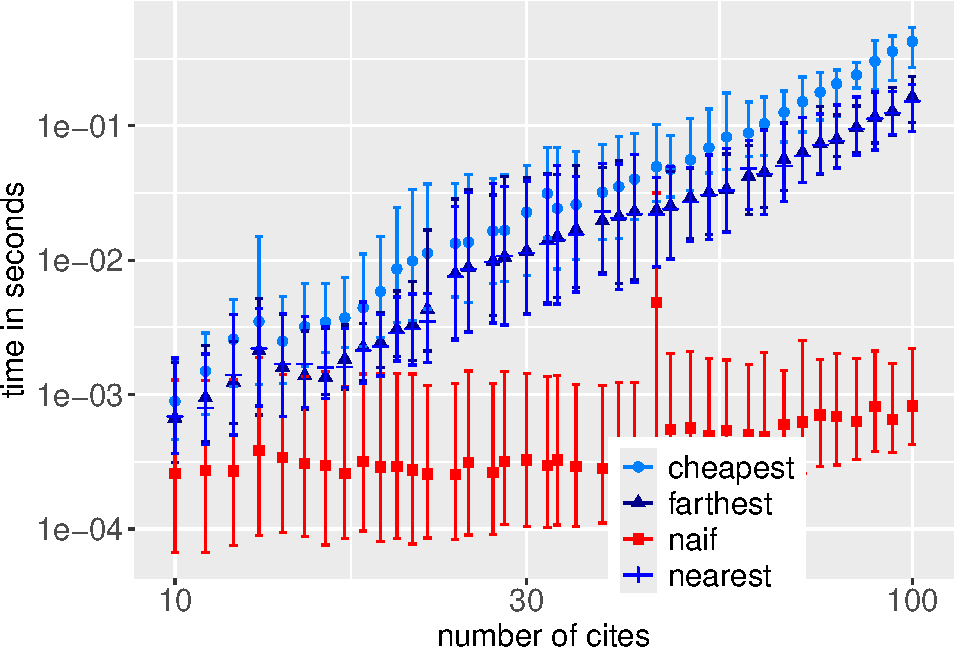
\includegraphics{TSP_analyse_files/figure-latex/unnamed-chunk-22-1.pdf}

On calcule les valeurs des coefficients directeurs.

\textbf{Pour naif :}

\begin{verbatim}
## (Intercept)      log(n) 
##  -9.6181451   0.5213248
\end{verbatim}

\textbf{Pour cheapest :}

\begin{verbatim}
## (Intercept)      log(n) 
##  -12.301360    2.452108
\end{verbatim}

\textbf{Pour nearest :}

\begin{verbatim}
## (Intercept)      log(n) 
##  -12.504142    2.298085
\end{verbatim}

\textbf{Pour farthest : }

\begin{verbatim}
## (Intercept)      log(n) 
##  -12.555933    2.318949
\end{verbatim}

\section{\texorpdfstring{Algorithme \emph{Branch and Bound} and
Programmation
Dynamique}{Algorithme Branch and Bound and Programmation Dynamique}}\label{algorithme-branch-and-bound-and-programmation-dynamique}

\begin{itemize}
\item
  Ajouter la fonction \texttt{B\_and\_B}
\item
  Ajouter la fonction \texttt{Held\_Karp} (programmation dynamique)
\item
  Evaluer le coefficient d'approximation des méthodes dans le cas d'une
  répartition uniforme et normale des villes
\end{itemize}

\section{Amélioration de tour par 2-opt et
3-opt}\label{amuxe9lioration-de-tour-par-2-opt-et-3-opt}

\textbf{EXERCIC Bonus :}

\begin{itemize}
\item
  Ajouter les fonctions \texttt{opt2} et \texttt{opt3} à coder
\item
  Evaluer l'amélioration apportée en terme de distance
\end{itemize}

\end{document}
